\documentclass[10pt,twocolumn]{article}
\usepackage[T1]{fontenc}
\usepackage{lmodern}
\usepackage[margin=0.58in,columnsep=0.22in]{geometry}
\usepackage{amsmath,amssymb,mathtools,bm}
\usepackage{tikz}
\usetikzlibrary{arrows.meta}
\usepackage{xcolor}
\usepackage{microtype}
\usepackage[colorlinks=true,linkcolor=blue!50!black,urlcolor=blue!50!black,citecolor=blue!50!black]{hyperref}

\setlength{\parindent}{0pt}
\setlength{\parskip}{1.5pt}
\setlength{\abovedisplayskip}{4pt}
\setlength{\belowdisplayskip}{4pt}
\setlength{\abovedisplayshortskip}{3pt}
\setlength{\belowdisplayshortskip}{3pt}
\allowdisplaybreaks
\sloppy
\raggedbottom

\newcommand{\ket}[1]{|#1\rangle}
\newcommand{\bra}[1]{\langle #1|}
\newcommand{\micro}[1]{\par\noindent\textbf{Micro-intuition:}\ #1\par}
\newcommand{\form}[1]{\par\noindent\textbf{Common mathematical form:}\ #1\par}
\newcommand{\commentary}[1]{\par\noindent\textbf{Commentary:}\ #1\par}
\newcommand{\phys}[1]{\par\noindent\textbf{Quantum-mechanical interpretation:}\ #1\par}
\newcommand{\geom}[1]{\par\noindent\textbf{Geometric visualization:}\ \textcolor{teal!70!black}{#1}\par}
\newcommand{\conceptbreak}{\par\medskip\noindent{\color{black!30}\rule{\columnwidth}{0.35pt}}\par\medskip}

\title{Joint Metric--Schur Batch Selection\\
\large A Unified Phase-III and Batch Derivation for Paper I}
\author{}
\date{}

\begin{document}
\maketitle
\vspace{-1.3em}

This note explains the new SNAKE batch selector after the reader has read
\emph{Metric-Regularized Schur Prune Response}. It reuses that note's
projector, Gram matrix, Hessian, pseudoinverse, and Schur conventions. Its main
purpose is manuscript verification: derive the joint selector, compare it
line by line with Phase III and batching in Paper I, and identify exactly which
parts coincide and which parts do not. Commentary accompanies the derivations;
it does not replace them.

\section*{Executive Reading}

The current ansatz prepares
\[
\ket{\psi}=U(\bm\theta)\ket{\phi_0}.
\]
A proposed batch \(B\) introduces one or more new Pauli-rotation coordinates.
The selector does not freeze the old angles while judging those rotations. It
models the old coordinates and proposed coordinates together, allows the old
ansatz to relax, and predicts the best local energy decrease.

The recurring objects are
\[
\boxed{\ket{\psi},\quad B,\quad g,\quad G,\quad H.}
\]
Here \(g\) is the local downhill energy vector, \(G\) is the Fubini--Study
Gram matrix, and \(H\) is the energy Hessian. Old ansatz coordinates are
labeled \(W\); proposed batch coordinates are labeled \(B\). The joint
coordinate is always
\[
z=
\begin{bmatrix}
\delta\theta_W\\
\alpha_B
\end{bmatrix}.
\]

The new selector can be read as
\[
\boxed{
(g,G,H)\longrightarrow(D(B),\nu(B))\longrightarrow J_\beta(B).
}
\]

This is the same elimination idea used by the prune route, but the physical
question is reversed:
The prune route forces a coordinate out and tests recovery. The batch route
introduces coordinates and predicts descent.

The unifying model developed in this note is
\begin{equation}
\boxed{
J_\beta(B)=D(B)\nu(B)^\beta.}
\label{eq:master-unified-value}
\end{equation}
Here \(D(B)\) is the conditional joint energy descent and \(\nu(B)\) is the
fraction of batch tangent volume that survives after quotienting out the active
ansatz span. The exponent \(\beta\) controls whether this novelty changes
ranking. The specialization coordinates are
\[
(|B|,\beta)=(1,1),\qquad(1,0),\qquad(s,0),\quad s\ge1.
\]
They correspond respectively to Phase III, the joint singleton selector, and
the joint batch selector. In the first case,
\(\nu(\{r\})=\mathcal N_3(r)\).

\begin{center}
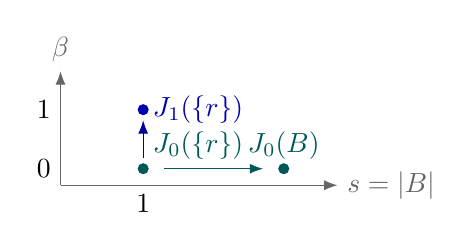
\begin{tikzpicture}[x=1.05cm,y=0.75cm,>=Latex]
  \draw[->,black!60] (0,-0.28) -- (3.35,-0.28) node[right] {$s=|B|$};
  \draw[->,black!60] (0,-0.28) -- (0,1.65) node[above] {$\beta$};
  \node[below] at (1,-0.28) {$1$};
  \node[left] at (0,0) {$0$};
  \node[left] at (0,1) {$1$};
  \fill[blue!70!black] (1,1) circle (2pt) node[right] {$J_1(\{r\})$};
  \fill[teal!70!black] (1,0) circle (2pt) node[above right] {$J_0(\{r\})$};
  \fill[teal!70!black] (2.7,0) circle (2pt) node[above] {$J_0(B)$};
  \draw[->,blue!60!black] (1,0.18) -- (1,0.82);
  \draw[->,teal!70!black] (1.25,0) -- (2.45,0);
\end{tikzpicture}
\end{center}
The vertical move turns explicit novelty weighting on for a singleton. The
horizontal move enlarges the same conditional-response model from one proposed
coordinate to a genuine batch.
The derivation below shows that these routes share the conditional energy
response. Their remaining differences arise from context, regularization, and
where the candidate population enters the construction.

\subsection*{What Is Reused from the Prune Note}

We reuse, without repeating their full derivations,
\[
\Pi=I-\ket{\psi}\bra{\psi},
\qquad
G_{ij}=\Re\langle\Pi\partial_i\psi,\Pi\partial_j\psi\rangle,
\]
the Moore--Penrose pseudoinverse \((\cdot)^+\), small ridge terms, symmetric
block structure, and Schur elimination. This avoids introducing a second notation
system for the same geometry.

\section*{Quantum Starting Point: Rays, Tangents, and Local Response}

\micro{The selector compares infinitesimal motions of a quantum ray, then uses
energy curvature to predict which finite local motion is worth admitting.}

A normalized vector and every globally rephased representative describe the
same physical pure state,
\[
\ket{\psi}\sim e^{i\varphi}\ket{\psi}.
\]
Pure states therefore inhabit projective Hilbert space. For
\(\ket{d\psi}=\sum_i z_i\partial_i\ket{\psi}\), the component parallel to
\(\ket{\psi}\) changes normalization or global phase rather than the physical
ray. Its horizontal representative is
\[
\ket{d\psi_\perp}=\Pi\ket{d\psi},
\qquad
\Pi=I-\ket{\psi}\bra{\psi}.
\]
At the current ray, the energy differential is a covector and the metric and
Hessian are symmetric bilinear forms:
\[
dE\in T_{[\psi]}^*\mathcal M,
\qquad
\mathsf g,\operatorname{Hess}E
\in\operatorname{Sym}^2(T_{[\psi]}^*\mathcal M).
\]
The arrays called \(g\), \(G\), and \(H\) are coordinate representations of
these different object types. A metric or response inverse is what converts
the covector \(dE\) into a tangent direction.
The Fubini--Study line element follows directly:
\begin{align*}
ds^2
&=\langle d\psi|d\psi\rangle
-|\langle\psi|d\psi\rangle|^2\\
&=\langle d\psi|\Pi|d\psi\rangle\\
&=\sum_{ij}z_i z_j
\Re\langle\partial_i\psi|\Pi|\partial_j\psi\rangle\\
&=z^{\mathsf T}Gz,
\end{align*}
with
\[
\boxed{G_{ij}=\Re\langle\Pi\partial_i\psi,
\Pi\partial_j\psi\rangle.}
\]

\form{This is a quotient-space metric represented as a Gram matrix.}

\commentary{The quotient identifies vectors differing only by global phase.
The projector realizes that quotient locally by selecting horizontal tangent
representatives. The Gram matrix converts coordinate coefficients into
physical lengths and angles. Its null directions are parameter changes that
create no first-order motion of the physical ray.}

\phys{Each selected generator supplies a controllable tangent of the many-body
state, and each proposed Pauli child supplies another. These tangents combine
coherently before their norm or energy is evaluated. The off-diagonal overlaps
therefore encode interference between quantum controls. A child can have a
large energy gradient yet add little new state motion when its tangent lies
nearly in the span already generated by the ansatz.}

\geom{Picture one ray as a point with horizontal tangent arrows emanating from
it. Global-phase motion has been collapsed by the quotient. The remaining
arrows form a local tangent plane, and \(z^{\mathsf T}Gz=\rho^2\) draws the
ellipsoid of equal physical state displacement in that plane.}

\conceptbreak

\subsection*{The Energy Functional on the Variational Manifold}

\micro{The metric tells how far the ray moves; the energy Taylor expansion
tells whether that motion descends.}

Use the downhill sign convention
\[
g_i=-\left.\frac{\partial E}{\partial z_i}\right|_{0},
\qquad
H_{ij}=\left.\frac{\partial^2E}
{\partial z_i\partial z_j}\right|_{0}.
\]
Then
\begin{align*}
E(z)
&=E(0)-g^{\mathsf T}z
+\frac12z^{\mathsf T}Hz+O(\|z\|^3),\\
\widehat{\Delta E}(z)
&:=E(0)-E(z)\\
&=g^{\mathsf T}z-\frac12z^{\mathsf T}Hz+O(\|z\|^3).
\end{align*}
If \(H\succ0\) and no trust constraint is active, the quadratic model gives
\begin{align*}
\nabla_z\widehat{\Delta E}(z)&=g-Hz=0,\\
z^\star&=H^{-1}g,\\
\widehat{\Delta E}(z^\star)
&=g^{\mathsf T}H^{-1}g
-\frac12g^{\mathsf T}H^{-1}HH^{-1}g\\
&=\frac12g^{\mathsf T}H^{-1}g.
\end{align*}

\form{This is a quadratic Taylor model and its Newton response.}

\commentary{The rightmost gradient is transformed by the inverse Hessian into
a coordinate response. The left gradient contracts with that response to
produce a scalar predicted descent. The repeated gradient expresses a
quadratic form, not two sequential applications. When a ridge, pseudoinverse,
or trust multiplier changes the solve, the final physical gain must still be
evaluated in the Taylor model containing \(H\).}

\phys{The Hamiltonian expectation defines an energy landscape over the
variational manifold. The gradient is the local downhill covector and the
Hessian describes how energetic response changes along the available quantum
controls. Inverse curvature weights a soft collective mode more strongly than
a stiff mode. This is a response of the controlled many-body state, rather
than spatial motion of a material object.}

\geom{Overlay energy contours on the Fubini--Study tangent ellipsoid. The
metric determines physical distance, while the Hessian rotates and stretches
the energy contours. The Newton response reaches the minimum of the local
quadratic surface; a trust region limits it to the neighborhood where that
surface remains credible.}

\conceptbreak

\section*{Short Classical Bridge: Force, Compliance, and Work}

\micro{A gradient acts like a generalized force, a curvature matrix acts like
a spring network, and the inverse curvature converts force into displacement.}

\form{This is the multidimensional version of a Hooke-law spring.}

Begin with one ordinary spring. If \(x\) is its displacement, \(F\) an applied
force, and \(k>0\) its stiffness, its local potential is
\[
E(x)=E(0)-Fx+\frac12kx^2.
\]
The equilibrium condition is
\[
kx^\star=F,
\qquad
x^\star=k^{-1}F.
\]
Thus the stiffness \(k\) maps displacement to force, while the compliance
\(k^{-1}\) maps force to displacement. Substituting the equilibrium
displacement gives
\[
\boxed{
\Delta E^\star
=\frac12F x^\star
=\frac12F(k^{-1}F).
}
\]

\commentary{The force has not been applied twice. The right copy of \(F\) is
first transformed by the compliance into the displacement \(x^\star\). The
left copy then forms the product \(F x^\star\), which is work. The factor
\(1/2\) appears because the restoring force of a linear spring grows from zero
to its final value as the spring is displaced. Its average value along the
path is one half of the final force.}

In many coordinates, the same equations become
\[
Qx^\star=f,
\qquad
x^\star=Q^+f,
\qquad
\boxed{\Delta E^\star=\frac12 f^{\mathsf T}Q^+f.}
\]
Here \(Q\) is the stiffness matrix and \(Q^+\) is the compliance matrix. The
expression naturally separates into
\[
\begin{aligned}
x^\star&=Q^+f,\\
w&=f^{\mathsf T}x^\star.
\end{aligned}
\]
The first line produces the displacement vector; the second contracts force
with displacement to produce scalar work.

The only correspondence retained from this bridge is
\[
dE\xrightarrow{\ A^+\ }z
\xrightarrow{\ (dE)^{\mathsf T}\ }(dE)^{\mathsf T}z.
\]
The quantum derivations in the remaining sections determine what the response,
distance, redundancy, and energy actually mean.

\section*{1. The Gram Matrix Is a Dot-Product Table}

\micro{Before asking which batch lowers the energy, ask whether its proposed
wavefunction motions are genuinely new and mutually distinct.}

\form{A Gram matrix is a table of pairwise inner products.}

Let \(\tau_i=\partial_{\theta_i}\ket{\psi}\) be an old ansatz tangent and
\(\xi_a=\partial_{\alpha_a}\ket{\psi}\) a proposed child tangent. Using the
projector inherited from the prune note, the full metric is
\[
G=
\begin{bmatrix}
G_{WW}&G_{WB}\\
G_{BW}&G_{BB}
\end{bmatrix},
\qquad
G_{ij}=\Re\langle\Pi t_i,\Pi t_j\rangle,
\]
where each \(t_i\) is either an old tangent \(\tau_i\) or a proposed tangent
\(\xi_a\).

\commentary{This is ordinary linear algebra in a physically chosen inner
product. A Euclidean Gram matrix compares arrows in ordinary space. Here the
arrows are derivatives of a quantum state, and the projector removes the
unobservable component parallel to the state itself. The diagonal entries say
how strongly each parameter moves the physical state. The off-diagonal entries
say how much two parameter changes produce the same motion.}

The physical distance of a joint update is the quadratic form
\[
ds^2=z^{\mathsf T}Gz.
\]
This is the first familiar form to remember: a symmetric matrix defines a
length, angle, or ellipsoid through \(z^{\mathsf T}Gz\).

\phys{A parameter is not valuable merely because its numerical derivative is
large. It is valuable when it moves the ray of the many-body state in a useful
direction. Global phase motion contributes nothing. A candidate that mostly
reproduces an existing ansatz tangent is also mostly redundant, even if its raw
energy gradient looks large. The full \(G_{WB}\) block detects this redundancy
against the current ansatz; \(G_{BB}\) detects redundancy inside the batch.}

\geom{Draw every projected state derivative as an arrow from the current point
in projective Hilbert space. The Gram matrix records all arrow lengths and
mutual angles. Redundant arrows lie nearly on top of one another. Independent
arrows span area or volume. The surface \(z^{\mathsf T}Gz=\rho^2\) is an
ellipsoid describing a fixed physical displacement of the state.}

\section*{2. Energy Uses a Quadratic Taylor Model}

\micro{The Gram matrix tells us what motion is new; the Hessian tells us how
the energy bends when we move in those directions.}

\form{This is the standard second-order Taylor approximation.}

With the sign convention that \(g\) points downhill,
\[
E(z)\approx E(0)-g^{\mathsf T}z+\frac12z^{\mathsf T}Hz.
\]
Therefore the predicted reduction is
\[
\boxed{
\widehat{\Delta E}(z)
=g^{\mathsf T}z-\frac12z^{\mathsf T}Hz.
}
\]

\commentary{The first term is linear benefit: move with the downhill slope.
The second term is curvature correction: the landscape may flatten, steepen,
or turn before that linear gain is realized. This is the same quadratic model
used in Newton methods, response theory, least-squares corrections, and local
stability analysis. The batching route is unusual only in what its coordinates
mean: some coordinates already belong to the ansatz, while others are proposed
Pauli rotations.}

Like \(G\), the Hessian is measured as one full block matrix:
\[
H=
\begin{bmatrix}
H_{WW}&H_{WB}\\
H_{BW}&H_{BB}
\end{bmatrix},
\qquad
g=
\begin{bmatrix}
g_W\\g_B
\end{bmatrix}.
\]

\phys{The mixed block \(H_{WB}\) describes energetic response between old and
new rotations. It is the local statement that introducing a new correlation
channel changes the best amplitudes of correlations already present. The
off-diagonal entries of \(H_{BB}\) describe cooperation or interference among
new children. A batch is therefore not scored by adding isolated singleton
gains; its collective curvature is part of the physical prediction.}

\geom{Imagine an energy surface drawn over the tangent plane. The gradient is
an arrow pointing down the surface. The Hessian determines whether the surface
is bowl-shaped, saddle-shaped, narrow, or flat. Off-diagonal entries rotate the
principal axes of that bowl. Ignoring them forces the contours to align with
the coordinate axes and erases genuine coupling.}

\section*{3. One Schur Formula Does All Elimination}

\micro{The old ansatz coordinates are nuisance variables for the selection
decision: they must be allowed to respond, but the final choice concerns the
new batch.}

\form{This is block Gaussian elimination, expressed as a Schur complement.}

Consider the generic linear system
\[
Ax=b,
\qquad
A=
\begin{bmatrix}
A_{WW}&A_{WB}\\
A_{BW}&A_{BB}
\end{bmatrix},
\qquad
b=
\begin{bmatrix}
b_W\\b_B
\end{bmatrix}.
\]
Eliminating the old coordinates \(W\) gives
\[
\boxed{
\widetilde A
=A_{BB}-A_{BW}A_{WW}^{+}A_{WB},
}
\]
\[
\boxed{
\widetilde b
=b_B-A_{BW}A_{WW}^{+}b_W.
}
\]
Solve \(\widetilde A x_B=\widetilde b\), then reconstruct
\[
x_W=A_{WW}^{+}(b_W-A_{WB}x_B).
\]

\commentary{This is not a specialized quantum formula. It is the same
operation used to eliminate latent variables in Gaussian models, internal
nodes in electrical networks, constrained coordinates in mechanics, and
nuisance regressors in least squares. The reduced matrix asks: after the old
variables respond as well as they can, what relation remains among the new
variables?}

The prune and batch routes differ in the constraint they impose, but both use
this same algebra. The batch route applies it twice with two familiar choices
of \(A\).

\subsection*{Geometric Use}

Set
\[
A=G+\epsilon I,
\qquad b=g.
\]
The generic formula removes descent already explainable by old ansatz motion.
The reduced solve produces a geometric batch direction \(d_B\), and
\[
\boxed{D_0=\widetilde b^{\mathsf T}d_B}
\]
is the raw Geo-ADAPT-style descent certificate.

\commentary{This quantity is reported before Hessian correction and trust
clipping. It answers the clean geometric question: does the proposed batch
contain downhill state motion outside the current ansatz tangent span?}

\subsection*{Finite-Energy Use}

Set
\[
A=H+\lambda G+\epsilon I,
\qquad b=g.
\]
The same three elimination equations produce the batch step \(\alpha_B\) and
the accompanying old-angle relaxation \(\delta\theta_W\). Together they form
the joint step \(z^\star\), which is inserted into the Taylor model:
\[
\boxed{
\widehat{\Delta E}(B)
=\max\left\{0,
g^{\mathsf T}z^\star
-\frac12(z^\star)^{\mathsf T}Hz^\star
\right\}.
}
\]

The elimination is performed on the combined matrix \(H+\lambda G\). In
general,
\[
\operatorname{Schur}(H+\lambda G)
\ne
\operatorname{Schur}(H)+\lambda\operatorname{Schur}(G).
\]

\commentary{This distinction matters because the inverse of a sum is not the
sum of inverses. Energy curvature and state-space geometry can couple old and
new directions differently. The trust multiplier must reshape the full joint
problem before the old coordinates are removed.}

\phys{Eliminating \(W\) does not freeze or discard the existing ansatz. It
models its best local response. The proposed child rotations perturb the
many-body wavefunction; the already-present hopping, displacement, and
interaction amplitudes then readjust. The selector credits the batch only for
the energy decrease remaining after this coherent relaxation is included.}

\geom{For every fixed batch displacement, slide along the old-coordinate
directions until reaching the bottom of that cross-section of the quadratic
bowl. The collection of these conditional minima forms a lower-dimensional
valley. The Schur complement is the curvature of that valley, and the reduced
gradient is its downhill slope.}

\section*{4. Trust Regions Are Constrained Quadratic Optimization}

\micro{A local Taylor model is useful only near the state where its derivatives
were measured.}

\form{This is the standard trust-region problem, but distance is measured by
the Fubini--Study metric.}

The accepted local model obeys
\[
(z^\star)^{\mathsf T}Gz^\star\le\rho^2.
\]
If the unconstrained step is too large or unstable, \(\lambda\) is increased
inside \(H+\lambda G\) until the step is regular and lies inside this region.

\commentary{The multiplier is not a new scoring term. It is a numerical and
physical safeguard. In Euclidean optimization, a trust region limits
\(\|z\|^2\). Here two parameter vectors with the same Euclidean norm can move
the quantum state by very different amounts, so \(z^{\mathsf T}Gz\) is the
appropriate local distance.}

\phys{The safeguard limits distinguishable wavefunction motion, not arbitrary
angle size. It is invariant to global phase and adapts to redundant or strongly
responsive coordinates. The raw certificate \(D_0\) remains
visible so that clipping does not hide whether a genuinely new downhill
direction existed before the finite-step safeguard was applied.}

\geom{The quadratic energy model is a bowl or saddle; the metric trust region
is an ellipsoid centered at the current state. The proposed Newton-like step
may lie outside the ellipsoid. Increasing \(\lambda\) bends and shortens the
step until it touches or enters the trusted geometric neighborhood.}

\conceptbreak

\section*{5. Paper-I Phase III and Joint Batching as One Story}

\micro{The singleton joint selector shares Phase III's Schur-relaxed energy
model under specific assumptions, while the complete Phase-III score contains
an additional multiplicative novelty factor.}

The corresponding source anchors in \texttt{Paper\_I.tex} are
\nolinkurl{eq:master_phase_score}, \nolinkurl{eq:local_quadratic},
\nolinkurl{eq:phase3_schur_response},
\nolinkurl{eq:phase3_star_geometry}, \nolinkurl{eq:phase3_novelty}, and
\nolinkurl{eq:batch_argmax}. The equations below preserve that notation while
making the hidden reductions explicit.

\subsection*{One Quotient-Space Construction}

The adjoint below is taken with respect to the real Fubini--Study inner
product. Let \(m\) be the active-coordinate count and \(s=|B|\).

\par\noindent\textbf{Mathematical derivation:}\par
\[
\mathcal T=\operatorname{ran}\Pi,
\qquad
T_W:\mathbb R^m\to\mathcal T,
\qquad
T_B^\star:\mathbb R^s\to\mathcal T.
\]
\begin{align}
G_{WW}&=T_W^\dagger T_W,
\notag\\
G_{WB}^\star&=T_W^\dagger T_B^\star,
\notag\\
G_{BB}^\star&=(T_B^\star)^\dagger T_B^\star,
\notag\\
P_W&=T_WG_{WW}^+T_W^\dagger,
\notag\\
Q_W&=I-P_W,
\notag\\
(T_B^\star)^\perp&=Q_WT_B^\star,
\notag\\
\Gamma_B
&=((T_B^\star)^\perp)^\dagger(T_B^\star)^\perp
\notag\\
&=(T_B^\star)^\dagger Q_WT_B^\star
\notag\\
&=G_{BB}^\star
-(G_{WB}^\star)^{\mathsf T}G_{WW}^+G_{WB}^\star,
\label{eq:batch-residual-gram}\\
\mathbf N(B)
&=(G_{BB}^\star)^{+/2}\Gamma_B
\notag\\
&\quad\times(G_{BB}^\star)^{+/2},
\label{eq:batch-novelty-operator}\\
\Gamma_Bv_j&=\nu_jG_{BB}^\star v_j,
\notag\\
0&\le\nu_j\le1,
\notag\\
\nu(B)
&=\left[\frac{\det\Gamma_B}{\det G_{BB}^\star}\right]^{1/s}
=\det\!\bigl(\mathbf N(B)\bigr)^{1/s},
\label{eq:batch-volume-novelty}\\
\nu(\{r\})
&=\frac{F^\star-(q^\star)^{\mathsf T}G_{WW}^+q^\star}{F^\star}
\notag\\
&=\mathcal N_3(r).
\notag
\end{align}

\form{Equation~\eqref{eq:batch-residual-gram} is simultaneously a Gram matrix
of residual vectors, a metric Schur complement, and the induced metric on the
quotient of proposed directions by the active tangent span.}

The spectrum \(\{\nu_j\}\) gives the surviving fraction of every collective
batch mode. The determinant takes their geometric mean. If \(\Gamma_B\) loses
rank, \(\nu(B)=0\); if \(G_{BB}^\star\) lacks the required rank, the coordinate
proposal is infeasible. The determinant ratio is invariant under nonsingular
mixing of the batch coordinates because its numerator and denominator acquire
the same squared basis determinant.

\begin{center}
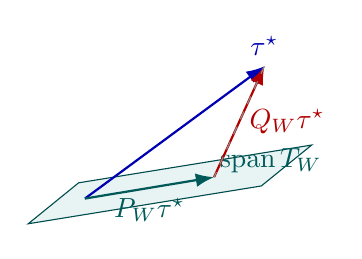
\begin{tikzpicture}[x=0.8cm,y=0.8cm,>=Latex]
  \fill[teal!9] (-0.3,-0.25) -- (3.4,0.35) -- (4.2,1.0) -- (0.5,0.4) -- cycle;
  \draw[teal!60!black] (-0.3,-0.25) -- (3.4,0.35) -- (4.2,1.0) -- (0.5,0.4) -- cycle;
  \node[teal!70!black] at (3.55,0.75) {$\operatorname{span}T_W$};
  \coordinate (O) at (0.6,0.15);
  \coordinate (P) at (2.65,0.49);
  \coordinate (T) at (3.45,2.25);
  \draw[->,thick,blue!70!black] (O) -- (T) node[above] {$\tau^\star$};
  \draw[->,thick,teal!70!black] (O) -- (P) node[midway,below] {$P_W\tau^\star$};
  \draw[->,thick,red!70!black] (P) -- (T) node[midway,right] {$Q_W\tau^\star$};
  \draw[dashed,black!45] (T) -- (P);
\end{tikzpicture}
\end{center}
The blue tangent decomposes into an active-span component and a quotient
component. For one record, \(\nu(\{r\})\) is the squared red length divided by
the squared blue length. For a batch, Eq.~\eqref{eq:batch-volume-novelty}
compares the corresponding tangent volumes.

\commentary{A scalar candidate has only one collective mode, so its novelty
operator has one eigenvalue and no scalarization ambiguity. A batch has several
modes. Equation~\eqref{eq:batch-volume-novelty} chooses their geometric mean,
equivalently the surviving tangent-volume fraction per proposed coordinate.
Other summaries answer different scientific questions, so this choice is a
modeling decision. It is nevertheless non-piecewise, coordinate invariant, and
reduces exactly to the Phase-III novelty fraction for one record.}

\phys{The active ansatz already controls a subspace of first-order many-body
motions. The columns of \((T_B^\star)^\perp\) are the portions of proposed
motions that cannot be synthesized by retuning those existing controls. The
eigenvectors of \(\mathbf N(B)\) are coherent superpositions of the proposed
Pauli rotations. An eigenvalue near zero identifies a collective combination
that is almost entirely reproducible by the present ansatz; an eigenvalue near
one identifies a combination that opens a nearly orthogonal response channel.}

\geom{Start with the parallelepiped spanned by the compensated batch arrows.
Project it orthogonally away from the active tangent plane. Its individual edge
lengths, angles, area, and volume all change. The scalar Phase-III novelty sees
the surviving squared length of one edge. The operator \(\mathbf N(B)\) records
the surviving fractions of every principal collective axis of the whole
projected figure.}

The common energetic object is the conditional value of enlarging the active
local model by the batch subspace:
\begin{equation}
\boxed{
D(B)
=\max_{\delta\theta_W,\alpha_B}\widehat{\Delta E}
(\delta\theta_W,\alpha_B)
-\max_{\delta\theta_W}\widehat{\Delta E}
(\delta\theta_W,0).}
\label{eq:conditional-enlargement-value}
\end{equation}
The same trust constraint is imposed in both maxima. At a fully reoptimized
current ansatz, the second term is locally zero. Equation
\eqref{eq:conditional-enlargement-value} makes the energy calculation a value
of subspace enlargement rather than a value assigned to coordinate labels. If
the proposed tangent subspace lies entirely inside the active tangent subspace
and the local model is represented consistently, the two feasible physical
subspaces coincide and \(D(B)=0\).

Combining the canonical energetic and geometric objects yields
\[
J_\beta(B)=D(B)\nu(B)^\beta,
\]
which is Eq.~\eqref{eq:master-unified-value}. This is the natural common
formulation: \(D(B)\) measures conditional energetic opportunity,
\(\nu(B)\) measures quotient-space volume novelty, and \(\beta\) specifies how
strongly explicit novelty influences selection.

\conceptbreak

Paper I multiplies energetic gain by geometric novelty before applying its
separate hardware-cost normalization. This note suppresses the cost denominator
and studies the value numerator
\begin{equation}
\boxed{\mathcal V^{(t)}(r)=\Delta E_t(r)\mathcal N_t(r).}
\label{eq:audit-master-score}
\end{equation}
For Phase III, a record \(r\) has scalar candidate amplitude \(\alpha\) and an
old-coordinate response \(\delta\theta_W\). In the manuscript notation,
\begin{align}
E(\alpha,\delta\theta_W)
\approx{}&E_0-g\alpha+\frac12h\alpha^2
+\alpha c^{\mathsf T}\delta\theta_W
+\frac12\delta\theta_W^{\mathsf T}R\delta\theta_W,
\label{eq:audit-phase3-local}\\
R={}&\frac12(H_{WW}+H_{WW}^{\mathsf T})+\lambda_HI\succ0.
\label{eq:audit-phase3-ridge}
\end{align}
The stationarity condition for the inherited coordinates is
\begin{align*}
\nabla_{\delta\theta_W}E
&=\alpha c+R\delta\theta_W=0,\\
\delta\theta_W^\star
&=-\alpha R^{-1}c.
\end{align*}
Substitution into Eq.~\eqref{eq:audit-phase3-local} gives
\begin{align*}
E(\alpha,\delta\theta_W^\star)-E_0
={}&-g\alpha+\frac12h\alpha^2
-\alpha^2c^{\mathsf T}R^{-1}c\\
&+\frac12\alpha^2c^{\mathsf T}R^{-1}RR^{-1}c\\
={}&-g\alpha
+\frac12\left(h-c^{\mathsf T}R^{-1}c\right)\alpha^2.
\end{align*}
Hence the Schur-relaxed curvature is
\begin{equation}
\boxed{h^\star=h-c^{\mathsf T}R^{-1}c,}
\label{eq:audit-phase3-hstar}
\end{equation}
and the Phase-III gain is
\begin{equation}
\Delta E_3(r)
=\max_{\substack{\alpha\ge0\\
\alpha\sqrt{F^\star}\le\rho}}
\left[g\alpha-\frac12[h^\star]_+\alpha^2\right].
\label{eq:audit-phase3-gain}
\end{equation}

\form{Equations~\eqref{eq:audit-phase3-local}--\eqref{eq:audit-phase3-gain}
are conditional quadratic minimization and a scalar Schur complement.}

\subsection*{Where Phase-III Novelty Enters}

The induced old-coordinate response changes the candidate tangent to
\begin{align}
\tau^\star
&=\tau-\sum_{i\in W}(R^{-1}c)_i\tau_i,\label{eq:audit-taustar}\\
F^\star
&=\Re\langle\Pi\tau^\star,\Pi\tau^\star\rangle,\\
q_i^\star
&=\Re\langle\Pi\tau_i,\Pi\tau^\star\rangle.
\end{align}
Projecting \(\tau^\star\) onto the old tangent span solves
\begin{align*}
\gamma^\star
&=\arg\min_\gamma
\left\|\Pi\left(\tau^\star-
\sum_{i\in W}\gamma_i\tau_i\right)\right\|^2,\\
G\gamma^\star&=q^\star,\\
\gamma^\star&=G^+q^\star.
\end{align*}
Expanding the residual norm at this solution gives
\begin{align*}
\left\|\Pi\left(\tau^\star-
\sum_i\gamma_i^\star\tau_i\right)\right\|^2
&=F^\star-2(\gamma^\star)^{\mathsf T}q^\star
+(\gamma^\star)^{\mathsf T}G\gamma^\star\\
&=F^\star-(q^\star)^{\mathsf T}G^+q^\star.
\end{align*}
Therefore Paper I defines
\begin{equation}
\boxed{
\mathcal N_3(r)
=1-\frac{(q^\star)^{\mathsf T}G^+q^\star}{F^\star},
\qquad
\mathcal V^{(3)}(r)
=\Delta E_3(r)\mathcal N_3(r).}
\label{eq:audit-phase3-score}
\end{equation}

The transition from additive geometry to multiplicative ranking has two
separate steps. Orthogonality first gives the Pythagorean identity
\begin{align*}
F^\star
&=\|\Pi\tau^\star\|^2\\
&=\|P_W\Pi\tau^\star\|^2
+\|Q_W\Pi\tau^\star\|^2.
\end{align*}
Normalization then converts the residual summand into a dimensionless fraction,
\[
\mathcal N_3(r)
=\frac{\|Q_W\Pi\tau^\star\|^2}{\|\Pi\tau^\star\|^2}.
\]
Finally, Paper I makes the independent selector choice
\[
\Delta E_3(r)
\longmapsto
\Delta E_3(r)\mathcal N_3(r).
\]
The multiplication is therefore not forced by the additive decomposition. The
decomposition supplies a normalized geometric observable; the selector chooses
to use that observable as a soft weight on energetic value.

\commentary{The novelty factor is a normalized residual squared norm. It asks
what fraction of the compensated candidate tangent remains outside the old
ansatz tangent span. It is an explicit multiplicative ranking factor. The mere
presence of \(G\) in a trust region, a rank test, or a regularized response
solve does not algebraically reproduce this multiplication.}

\phys{Phase III distinguishes two questions. The Schur energy calculation asks
how much the Hamiltonian expectation can fall after the old amplitudes respond.
The novelty calculation asks how much of the resulting state motion remains a
new controllable direction rather than a re-expression of motion already
available. A candidate may receive a favorable energetic prediction while
still being down-weighted because its tangent response is largely redundant.}

\geom{First slide along the old-coordinate directions to obtain the
Schur-relaxed tangent \(\tau^\star\). Then orthogonally project that arrow onto
the old tangent span. The residual arrow supplies the numerator of
\(\mathcal N_3\); its ratio to the full \(\tau^\star\) length is the surviving
fraction. Schur relaxation and novelty projection are two distinct geometric
operations.}

\subsection*{The Singleton Reduction of the New Joint Model}

For one proposed record, write the unregularized joint Hessian as
\[
H=\begin{bmatrix}R&c\\c^{\mathsf T}&h\end{bmatrix},
\qquad
g_z=
\begin{bmatrix}g_W\\g\end{bmatrix}.
\]
At an exactly reoptimized current ansatz, \(g_W=0\). The block stationarity
equations become
\begin{align*}
R\delta\theta_W+c\alpha&=0,\\
c^{\mathsf T}\delta\theta_W+h\alpha&=g.
\end{align*}
The first gives \(\delta\theta_W=-R^{-1}c\alpha\); inserting it into the
second gives
\begin{align*}
\left(h-c^{\mathsf T}R^{-1}c\right)\alpha&=g,\\
\alpha^\star&=(h^\star)^+g.
\end{align*}
Define the reconstruction map
\[
T=\begin{bmatrix}-R^{-1}c\\1\end{bmatrix},
\qquad z=T\alpha.
\]
Then the physical metric along the relaxed singleton direction is
\begin{align*}
z^{\mathsf T}G_z z
&=\alpha^2T^{\mathsf T}G_zT\\
&=\alpha^2\left[
F-2q^{\mathsf T}R^{-1}c
+c^{\mathsf T}R^{-1}G R^{-1}c
\right]\\
&=\alpha^2F^\star.
\end{align*}
Thus the energy Schur curvature and metric trust constraint coincide with the
Phase-III singleton construction when the same coordinate window \(W\) and
response block \(R\) are used, and
\[
\boxed{
\begin{gathered}
B=\{r\},\quad g_W=0,\\
\lambda=0
\end{gathered}}
\]

The cost-suppressed values nevertheless remain
\begin{align*}
J_0(\{r\})
&=D(\{r\}),\\
J_1(\{r\})
&=D(\{r\})\nu(\{r\})
=\Delta E_3(r)\mathcal N_3(r).
\end{align*}
These are equal only if \(\mathcal N_3(r)=1\), or if the new route explicitly
restores the same novelty multiplier.

If the new route solves with \(H+\lambda G\), it eliminates the combined
system:
\begin{equation}
\overline M_{BB}(\lambda)
=M_{BB}-M_{BW}M_{WW}^+M_{WB},
\qquad M=H+\lambda G.
\label{eq:audit-combined-schur}
\end{equation}
This generally differs from first forming \(h^\star\) from \(H\) and then
using \(F^\star\) only as a trust boundary. Hence active metric damping is a
second source of non-equivalence.

\form{This is a limiting-case reduction: a shared subcalculation does not imply
identity of the complete scoring maps.}

\subsection*{Paper-I Batching and the New Placement of Batching}

Paper I first applies Phase III to individual records and then chooses a batch
from the retained set \(\mathcal R_k^{(3)}\). Suppressing the separate cost
denominator, its geometric-energy content is
\begin{align*}
H_B^\star
&=H_{BB}-H_{BW}R_B^{-1}H_{WB},\\
\Delta E_3(B)
&=\max_{\substack{\alpha_B\succeq0\\
\alpha_B^{\mathsf T}G_B^\star\alpha_B\le\rho_B^2}}
\left[g_B^{\mathsf T}\alpha_B
-\frac12\alpha_B^{\mathsf T}H_B^\star\alpha_B\right],\\
B^\star
&\in\arg\max_{B\subseteq\mathcal R_k^{(3)}}
\Delta E_3(B).
\end{align*}
There is no second explicit batch novelty multiplier in this objective.
Novelty has already affected which records survived Phase III.

The new route maps child Phase-II survivors directly into the joint
singleton/batch evaluator, so it skips the individual Phase-III multiplication
by \(\mathcal N_3(r)\).
Its optional additivity defect,
\[
d(B)
=\max\!\left\{0,
1-\frac{D(B)}
{\sum_{r\in B}D(\{r\})+\epsilon}
\right\},
\]
measures collective nonadditivity. It does not measure residual tangent novelty
relative to the old ansatz and is not a replacement for \(\mathcal N_3\).

\subsection*{Would a Batch Novelty Multiplier Double-Count Geometry?}

The joint solve and the novelty operator use the same tangent data for different
mathematical purposes. The scalar \(D(B)\) is the best descent after active
relaxation. The scalar \(\nu(B)\) is the surviving tangent-volume fraction.
Exact redundancy is already removed by the quotient construction and should
give no new energetic subspace. Rank and conditioning rules can also reject an
ill-posed batch. Multiplying by \(\nu(B)^\beta\) adds a further soft
preference among the remaining well-defined subspaces. It therefore preserves
independent geometric information, but it deliberately weights redundancy a
second time in the policy after redundancy has already influenced feasibility
and response.

There is no universal yes-or-no answer. With \(\beta=0\), geometry determines
the trusted response and feasibility but does not impose a separate novelty
preference. With \(\beta=1\), selection additionally favors subspaces whose
collective tangent volume survives strongly in the quotient. For one record,
this is exactly the Phase-III novelty multiplier. For a batch, it is the
coordinate-invariant volume generalization in
Eq.~\eqref{eq:batch-volume-novelty}.

\phys{The current manuscript uses novelty as a record-level gate before the
collective energetic contest. The new route lets the collective quantum
response itself decide among Phase-II survivors. This can preserve a pair whose
members are modest individually but useful together, while also removing the
explicit soft preference for individually novel tangents. The two routes make
different scientific choices even though both use Gram matrices and Schur
relaxation.}

\geom{Paper I first shrinks the cloud of candidate arrows by coloring each
arrow according to its residual length, then forms subsets from the surviving
cloud. The new route forms subset subspaces directly from the Phase-II cloud
and compares their reduced energy surfaces. The paths meet at the joint Schur
model but arrive there through different filters.}

\subsection*{Diagnostic Limiting Cases}

The unified objects make the principal limits explicit:
\begin{center}
\begin{tabular}{p{0.27\columnwidth}p{0.57\columnwidth}}
\textbf{Geometry} & \textbf{Consequence}\\\hline
\(T_B^\star\subseteq\operatorname{span}T_W\)
&\(\Gamma_B=0\), \(\nu(B)=0\), and a consistent conditional-enlargement
model gives \(D(B)=0\).\\
\((T_W)^\dagger T_B^\star=0\)
&\(\Gamma_B=G_{BB}^\star\) and \(\nu(B)=1\): every batch mode
is fully novel relative to the active span.\\
\(\operatorname{rank}\Gamma_B<|B|\)
&At least one collective batch combination is redundant after quotienting;
its novelty eigenvalue is zero.\\
\(\Gamma_B\) full rank
&The batch adds \(|B|\) independent quotient directions, but its energy need
not be additive because \(H_{BB}\) may have off-diagonal coupling.\\
\(H_{WB}=G_{WB}=0\)
&Active-coordinate Schur corrections vanish; old coordinates do not respond
to the batch in the local model.\\
\(b=1\)
&The matrix novelty spectrum has one value and the joint response becomes the
scalar Schur model derived above.
\end{tabular}
\end{center}

The fourth line is especially important. Metric independence does not imply
energetic independence. Even when \(G_{BB}\) is diagonal, an off-diagonal
Hessian element contributes
\[
-\frac12\sum_{a\ne b}\alpha_a(H_{BB})_{ab}\alpha_b
\]
to the predicted descent. This cooperation or interference is why
\(D(B)\) generally differs from
\(\sum_{r\in B}D(\{r\})\).

\section*{6. Joint Feasibility and Nonadditivity}

\micro{Remove duplicate directions first, reject geometrically invalid subsets
second, and only then compare scores.}

A canonical child identity is the normalized Pauli word together with its
insertion position. Overall sign or irrelevant global phase does not create a
new direction. The same child generated by different parent macros becomes one
record, while every parent label is retained as provenance. Different positions
remain alternative records, but two positions of the same exact child cannot
coexist in one batch. Distinct siblings from one parent may coexist.

\form{Rank tests check independence; condition numbers check numerical
stability.}

After old-ansatz motion is eliminated, a batch must retain the requested rank
and acceptable conditioning. Rank failure means the batch contains fewer
independent state directions than parameters. Poor conditioning means tiny
measurement changes can create large changes in the inferred amplitudes.

\commentary{These are hard feasibility tests because an unstable coordinate
system cannot support a trustworthy local solve. Additivity is different. It
asks whether the joint predicted gain falls below the sum of contextual
singleton gains. That is evidence of interference or model uncertainty, not
proof that the batch is impossible.}

With minimal extra notation, the optional soft defect is
\[
d(B)=\max\left\{0,
1-\frac{D(B)}
{\sum_{r\in B}D(\{r\})+\epsilon}
\right\},
\]
and the softened energetic value is
\[
\widetilde J(B)
=\frac{D(B)}{1+\lambda_a d(B)}.
\]
Setting \(\lambda_a=0\) recovers the exact joint energetic value. The defect
does not replace the joint Gram/Hessian calculation and does not act as a
canonical hard rejection.

\phys{A large defect means that attractive isolated responses interfere when
the rotations are introduced together. The batch may still encode a useful
many-body process, so it remains eligible. The soft factor expresses reduced
confidence without declaring the collective direction physically forbidden.}

\geom{The sum of singleton gains defines an additive reference height. The
joint model produces the actual point. Their vertical shortfall is the defect.
A soft penalty smoothly lowers that region of the score surface; a hard gate
would instead cut an artificial cliff through it.}

\section*{Compact Reading Summary}

The new route is built from common forms rather than unrelated formulas.
The Gram matrix supplies physical lengths and angles; the Taylor quadratic
supplies local energy prediction; the Schur complement eliminates active-angle
response; the trust region limits physical state displacement; and the
residual Gram spectrum records which collective quotient directions survive.

The central physical statement is equally compact: a proposed batch is judged
not as a collection of isolated gradients, but as a joint enlargement of the
current variational manifold. The old ansatz relaxes, the new directions
interfere through full Gram and Hessian blocks, and the surviving predicted
energy descent may or may not receive an additional explicit novelty weight.

\section*{Worked Reading: One Candidate Pair}

Suppose the search considers a pair \(B=\{r_1,r_2\}\). Nothing new must be
invented to understand the calculation. The pair selects two proposed
coordinates from the full joint local model.

\micro{Read the pair as two new arrows judged in the presence of every old
ansatz arrow.}

First, global identity processing has already ensured that \(r_1\) and
\(r_2\) are distinct physical records and are compatible in one batch. Their
parent labels are provenance, not coordinates. If both records came from one
parent macro, that does not make them redundant. If they are two insertion
positions of the same exact child, compatibility rejects the pair before the
matrix solve.

Second, the two-by-two block \(G_{BB}\) compares the candidate tangents with
one another. The mixed block \(G_{WB}\) compares both candidates with the
whole active ansatz. A pair can look independent inside \(G_{BB}\) yet become
redundant after old-ansatz motion is removed. This is the familiar distinction
between ordinary independence and independence modulo an existing subspace.

Third, the Hessian blocks ask a different question. Even when both state-space
directions survive the metric test, their energetic effects can cooperate or
compete. A negative or favorable mixed curvature can make the pair better than
its isolated members suggest. Unfavorable interference can make the joint gain
smaller than the singleton sum. In both cases the joint quadratic form, not an
additive shortcut, supplies the prediction.

\commentary{The Schur step now has a simple verbal reading. For the proposed
pair, let every old angle make its best local compensating response. Remove
that response from the equations. What remains is a two-coordinate problem
describing only the pair's irreducible effect beyond the present ansatz. Solve
that small problem, then reconstruct how the old angles moved with it.}

Fourth, the reconstructed update is checked against the same Fubini--Study
trust ellipsoid. If the predicted motion leaves the local neighborhood,
\(\lambda\) contracts the coupled old-plus-new response. The pair is not
penalized merely for containing two records; it is constrained according to
how far the complete update moves the physical state.

Finally, insert the reconstructed step into the energy Taylor model. Compare
its joint energetic value with every compatible singleton and larger allowed
subset. If an explicit novelty policy is active, apply
\(\nu(B)^\beta\) only after the joint gain and novelty spectrum have
been computed separately.

\phys{A useful pair is therefore not simply ``two strong gradients.'' It is two
new controllable quantum motions that remain distinct from the current ansatz,
interact favorably enough in the local energy landscape, stay within the
trusted state-space neighborhood, and survive the chosen novelty policy.}

\geom{Begin with a cloud of old tangent arrows and two candidate arrows.
Project away the old cloud, leaving two residual arrows. Their angle and length
define a small metric ellipse. Lay the reduced energy contours over that
ellipse, find the downhill point inside the trusted boundary, and then place
the resulting pair on the energy-versus-novelty plane. These are successive
views of the same two-coordinate proposal.}

\section*{How to Read \(v^{\mathsf T}A^{+}v\) at a Glance}

\micro{Read from right to left to obtain a vector, then finish with the left
vector to obtain a scalar.}

Whenever an expression has the form
\[
\frac12v^{\mathsf T}A^+v,
\]
use the following four-step visual reading.

\textbf{1. Identify the input vector.}
The rightmost \(v\) is the applied generalized force. It has a magnitude and a
direction in coordinate space.

\textbf{2. Apply the linear map.}
Compute
\[
x=A^+v.
\]
The matrix mixes and rescales the force components. If \(A\) is stiffness,
\(A^+\) is compliance and \(x\) is displacement. In an eigenvector basis, each
force component is divided by the corresponding supported stiffness.

\textbf{3. Form the dot product.}
The remaining expression is
\[
v^{\mathsf T}x.
\]
This is not another matrix transformation. It measures alignment between force
and displacement and sums that aligned response into one scalar.

\textbf{4. Interpret the factor \(1/2\).}
For an unconstrained linear restoring system, the force increases linearly
along the displacement path. The average restoring force is half its final
value, giving the familiar elastic-energy factor.

\commentary{A useful type check is
\[
v\xrightarrow{\ A^+\ }x
\xrightarrow{\ v^{\mathsf T}(\cdot)\ }v^{\mathsf T}x.
\]
If an explanation describes the final result as another direction, it has
missed the dot product. If it describes \(A^+\) as the stiffness rather than
the compliance, it has reversed the map.}

\subsection*{The Same Checklist in the Quantum Route}

For the quantum selector, the rightmost vector is an energy-gradient force.
The inverse response operator produces a parameter displacement. Those
parameter changes generate one coherent tangent-state displacement. The final
dot product measures how strongly the displacement follows the downhill
energy force.

The parameter-space map is \(g\mapsto z^\star\). The corresponding
projective-state tangent is
\[
z^\star\longmapsto
\Pi\sum_i z_i^\star\partial_i\ket{\psi}.
\]
The first is controlled by the response solve; the second is measured by the
Fubini--Study Gram matrix.

\phys{The parameter vector is not itself the wavefunction motion. It specifies
how much each quantum control changes. The tangent vectors translate those
control changes into a coherent state variation. Two very different parameter
vectors can represent nearly the same state motion when the tangent directions
are redundant. This is why the Gram matrix is essential rather than cosmetic.}

\geom{First draw the force arrow in parameter coordinates. Let the inverse
response matrix rotate and stretch it into a displacement arrow. Then map that
arrow through the tangent vectors into projective Hilbert space. The first
ellipsoid visualizes energetic or regularized response; the second visualizes
physical state distance. The same coefficients appear in both pictures, but
the matrices answer different questions.}

\subsection*{Common Interpretation Errors}

\textbf{Stiffness versus compliance.}
\(A\) maps displacement to force; \(A^+\) maps force to displacement.

\textbf{Two appearances of the force.}
The right appearance creates the displacement. The left appearance takes a dot
product with that displacement. It is not a second application of force.

\textbf{Gram matrix versus Hessian.}
\(G\) measures quantum-state distance and tangent redundancy. \(H\) measures
energy curvature. Both are symmetric quadratic forms, but they encode
different physics.

\textbf{Schur reduction versus deletion.}
Eliminating old coordinates means allowing them to relax analytically. It does
not remove those coordinates from the actual ansatz.

\textbf{Regularized solve versus physical energy.}
When \(H+\lambda G+\epsilon I\) chooses the step, the final predicted energy
must still be evaluated with the physical Taylor model containing \(H\). The
simple half-work identity is exact only in its unconstrained quadratic limit.

\commentary{The shortest correct sentence is: the inverse response turns a
generalized force into a displacement, the dot product turns force and
displacement into scalar work, and the quantum metric tells us what that
displacement means for the physical state.}

\conceptbreak

\section*{Reader Work: Verify the Unification}

Do not calculate long matrix inverses. Answer by identifying the governing
object, assumption, or limiting case.

\textbf{1. Additive geometry versus multiplicative policy.}
Explain why the Pythagorean decomposition of \(\tau_r^\star\) does not by
itself imply that \(\Delta E_3(r)\) must be multiplied by
\(\mathcal N_3(r)\). Identify the mathematical step and the policy step.

\textbf{2. Singleton repair.}
A draft claims that \(b=1\) automatically makes the new route identical
to Phase III. Give the smallest set of missing qualifications needed to repair
the claim.

\textbf{3. Batch novelty.}
Two novelty eigenvalues are close to one and a third is close to zero. Describe
the collective tangent geometry. Then explain why the scalar Phase-III novelty
formula alone does not tell you whether to use the minimum, mean, or product of
those eigenvalues.

\textbf{4. Geometry versus energy.}
Construct a verbal case in which two residual batch tangents are mutually
orthogonal but their joint energy value is not the sum of their singleton
values. Name the matrix block responsible.

\textbf{5. Manuscript decision.}
State the scientific difference between choosing \(\beta=0\) and \(\beta=1\) in
Eq.~\eqref{eq:master-unified-value}. Explain when the latter would amount to a
deliberate second preference for novelty rather than an algebraic necessity.

\clearpage
\section*{Entrance Quiz: From Metric--Schur Pruning to Batching}

This detachable quiz checks the conceptual prerequisites for this batching
note. Choose the strongest answer and briefly record why it is stronger than
the nearest alternative. The answer key is on the final page.

\textbf{1. Redundant tangent coordinates.}
Two coordinate perturbations generate the same horizontal state tangent at the
current quantum ray. Which statement best describes the Gram matrix?

\textbf{A.} It is singular because distinct coordinate labels fail to define
distinct physical tangent directions.\quad
\textbf{B.} It remains invertible, but its determinant becomes sensitive to
the chosen parameter scale.\quad
\textbf{C.} It becomes indefinite because one perturbation must be assigned a
negative norm.\quad
\textbf{D.} It stays positive definite after projecting away global phase,
because horizontal projection removes all redundancy.

\textbf{2. Supported inverse versus ridge.}
A metric has one well-resolved tangent mode and one numerically unresolved
mode. Which distinction is mathematically decisive?

\textbf{A.} A supported pseudoinverse retains the unresolved mode with a small
reciprocal, whereas a ridge deletes it.\quad
\textbf{B.} A supported pseudoinverse defines the resolved quotient; a ridge
changes the response assigned to retained modes and is a regularized model.\quad
\textbf{C.} Both operations are identical whenever the original matrix is
positive semidefinite.\quad
\textbf{D.} A ridge determines physical rank, while a supported pseudoinverse
only improves conditioning.

\textbf{3. Meaning of Schur elimination.}
In a prune-response model, retained coordinates \(W\) are eliminated before
the candidate deletion coordinate is judged. What has happened?

\textbf{A.} The retained coordinates have been frozen at their current values,
so only the deleted coordinate contributes.\quad
\textbf{B.} Their locally optimal response has been solved and substituted
back, leaving a reduced model for the deletion question.\quad
\textbf{C.} Their tangent directions have been projected out of Hilbert space,
so they cannot respond after the deletion.\quad
\textbf{D.} Their Hessian block has been replaced by the Gram block to enforce
state-space recovery.

\textbf{4. Metric and Hessian roles.}
Why can the Fubini--Study Gram matrix and the energy Hessian not be exchanged in
the local model?

\textbf{A.} The Gram matrix measures physical state displacement, while the
Hessian measures variation of the energy differential along coordinate
directions.\quad
\textbf{B.} The Gram matrix is always exact, while the Hessian is always a
statistical estimate.\quad
\textbf{C.} The Hessian measures physical state displacement, while the Gram
matrix supplies energetic stiffness.\quad
\textbf{D.} They differ only by the choice of pseudoinverse threshold.

\textbf{5. Residual novelty.}
A candidate tangent has a large raw norm but lies almost entirely in the span
of retained tangents. What should its Schur residual Gram contribution report?

\textbf{A.} Large novelty, because its unprojected tangent norm is large.\quad
\textbf{B.} Small novelty, because the retained span can synthesize nearly the
same physical direction.\quad
\textbf{C.} Indefinite novelty, because projection changes the tangent's
orientation.\quad
\textbf{D.} Unchanged novelty, because Schur reduction affects energy response
but not state geometry.

\textbf{6. Metric trust region.}
What does \(z^{\mathsf T}Gz\leq\rho^2\) control?

\textbf{A.} The Euclidean size of the parameter array independently of its
effect on the state.\quad
\textbf{B.} The local Fubini--Study displacement of the variational quantum
ray represented by the coordinate step.\quad
\textbf{C.} The maximum energy decrease permitted by the Hessian model.\quad
\textbf{D.} The fraction of the candidate tangent orthogonal to the retained
span.

\textbf{7. Prediction and validation.}
A Schur prune model predicts negligible energy loss, but the refitted pruned
ansatz has unacceptable realized energy. What follows?

\textbf{A.} The model prediction overrides the refit because it used
second-order information.\quad
\textbf{B.} The deletion is accepted after shrinking the metric ridge.\quad
\textbf{C.} The proposal is rejected and the pre-deletion state is restored;
the prediction was a local admission model, not final evidence.\quad
\textbf{D.} The deleted tangent is reclassified as a numerically null mode.

\textbf{8. From prune to batch.}
Which structural change converts the prune-response construction into the
batch-selection question developed in this note?

\textbf{A.} Replace state-space geometry by a purely energetic Hessian ranking.\quad
\textbf{B.} Reverse the conditional question: introduce a proposed tangent
block and ask for its best descent after retained coordinates relax.\quad
\textbf{C.} Hold retained coordinates fixed and sum the singleton gradient
magnitudes.\quad
\textbf{D.} Interpret every removed coordinate as a future batch candidate.

\subsection*{Jargon and High-Level Vocabulary}

\textbf{9. Bilinear form.}
Which use most precisely distinguishes a bilinear form from a quadratic form?

\textbf{A.} A bilinear form compares two independently variable vectors; its
same-vector restriction is a quadratic form. \quad
\textbf{B.} A bilinear form accepts one vector and returns another, while a
quadratic form returns a scalar. \quad
\textbf{C.} A bilinear form is an indefinite quadratic form written without a
matrix. \quad
\textbf{D.} A bilinear form is a linear functional restricted to a tangent
subspace.

\textbf{10. Covector.}
In the local energy model, what makes the gradient differential a covector?

\textbf{A.} It assigns a scalar first-order energy change to each tangent
displacement. \quad
\textbf{B.} It assigns a tangent displacement to each scalar energy change. \quad
\textbf{C.} It measures the squared physical length of a tangent displacement. \quad
\textbf{D.} It projects a candidate tangent orthogonally away from the active
span.

\textbf{11. Quotient space.}
What is being identified in the coordinate quotient induced by a singular Gram
matrix?

\textbf{A.} Energy models that have the same Hessian eigenvalues. \quad
\textbf{B.} Coordinate perturbations whose difference produces no supported
physical tangent. \quad
\textbf{C.} Quantum states with the same variational energy but different
fidelity. \quad
\textbf{D.} Candidate batches that have the same resource cost.

\textbf{12. Conditioning.}
What does poor conditioning of a retained solve mean?

\textbf{A.} The objective necessarily contains negative curvature. \quad
\textbf{B.} Small perturbations in the supplied data can cause large changes in
the solved response because retained spectral scales are widely separated. \quad
\textbf{C.} The retained directions are exactly redundant and must all be
deleted. \quad
\textbf{D.} The Schur complement has been formed in the wrong block order.

\clearpage
\section*{Entrance-Quiz Solutions}

\textbf{1. A.} Coordinate labels can be distinct while their horizontal
tangents coincide. The Gram matrix records the latter, so the duplicate
combination is a null direction.

\textbf{2. B.} Spectral support selection declares which quotient directions
are represented. A ridge modifies the response on that support and must remain
visible as regularization.

\textbf{3. B.} Schur reduction solves the retained-coordinate stationarity
condition and substitutes the result into the full model. The coordinates are
optimized out rather than physically erased.

\textbf{4. A.} Both are symmetric bilinear forms, but they answer different
questions: state-space length versus energy response.

\textbf{5. B.} Novelty is the norm or volume left after the old span receives
its best opportunity to explain the candidate direction.

\textbf{6. B.} The quadratic form is the local projective-Hilbert-space line
element. Equal raw coordinate norms need not imply equal physical motion.

\textbf{7. C.} A local model proposes a structural edit. Realized refit and
rollback preserve the scientific acceptance boundary.

\textbf{8. B.} The same conditional-response algebra is reused with the
physical question reversed: deletion asks recoverability; admission asks
additional trusted descent.

\textbf{9. A.} A bilinear form accepts two independent inputs and is linear in
each. A quadratic form evaluates the associated form on the same vector twice.

\textbf{10. A.} The differential lives in the dual tangent space: it consumes
a tangent vector and returns its first-order scalar energy response.

\textbf{11. B.} The quotient groups coordinate arrays that differ only by a
Gram-null combination, because they represent the same supported physical
motion.

\textbf{12. B.} Conditioning describes sensitivity, not the sign of curvature
or exact rank by itself. A small retained spectral scale can amplify small
input errors in the response.

\end{document}
